\chapter{Background}

\section{JavaScript}
\label{sec:es6-design}
\label{sec:imp-dep-behavior}

\js{} engines are virtual machines that parse source code,
compile it in bytecodes, and run these bytecodes. These engines
implement some version of the ECMAScript (\es{}), which emerged with
the goal to standardize variants of the language, such as Netscape's
JavaScript and Microsoft's JScript\footnote{The name JavaScript still
  prevails today, certainly for historical reasons.}. The \es{}
specification is regulated by Ecma International~\cite{es6-website}
under the TC39~\cite{tc39-github} technical committee.  Every year, a
new version of the \es{} specification is produced with new features
and minor fixes. The canonical spec today is
ES6~\cite{ecmas262-spec-repo,ecmas262-spec}.

%% In the following, we briefly describe different sources of
%% discrepancies that can emerge across different engine implementations
%% as results of the active changes in the \es{} specification.
%% .........
%% A compatibility table relating features and supporting engines is
%% publicly available~\cite{kangax}.

The specification of JavaScript is incomplete for different
reasons. Certain parts of the specification are undefined; it is
responsibility of engineers to decide how to implement these
functionalities. The JavaScript spec uses the label
``implementation-dependent'' to indicate these cases, where behavior
may differ from engine to engine. One reason this flexibility in the
spec exists is to enable compiler optimizations. For example, the
\js\ \mcodeid{for-in} loop construct does not clearly specify the
iteration order of
elements~\cite{so-forin-undefined,javascript-in-chrome} and different
engines capitalize on that for loop
optimizations~\cite{for-in-undefined}.  As another example, the
specification states that if the \mcodeid{Number.toPrecision()}
function is called with multiple arguments then the floating-point
approximation is
implementation-dependent~\cite{es6-toPrecision}. Various other cases
like these exist in the specification. Given the speed the
specification changes and the complexity of the language some features
are not fully implemented as can be observed by the Kangax
compatibility table~\cite{kangax}.  It is also worth noting that, as
in other languages, some elements in JS have non-deterministic
behavior (\eg{}, \mcodeid{Math.random} and \mcodeid{Date}). A test
that make decisions based on these elements could, in principle,
produce different outcomes on different runs. Carefully-written test
cases should not manifest this kind of flaky behavior.  As previously
mentioned, all those aspects make testing \js\ engines challenging.


%\subsection{Randomness}


%\subsection{\Fix{Other}}

%% 1) The stack depth in JS is often close to the real (native) C stack
%% depth, nevertheless observable by JS through recursion. This causes
%% differential behavior even on the same engine when JITs are enabled or
%% disabled, as the stack frame sizes vary. LangFuzz in particular
%% produces a lot of recursions and hits these problems even more often
%% than jsfunfuzz.\Mar{ask C. Holler. it is unclear to me how the output
%%   could be different.}

%% \section{Objects of Study}
%% This section discusses the objects we used in our study.

\section{Engines Studied}
\label{sec:methodology}
\label{sec:methodology:engines}~We selected 
JS engines according to the following criteria: 1) Released latest
version after Jan 1, 2018, 2) Contains more than 1K stars on GitHub,
and 3) Uses a public issue tracker. We looked for highly-maintained
(as per the first criterion) and popular (as per the second criterion)
engines. As we wanted to report bugs, we also looked for project with
public issue trackers. Table~\ref{tab:engines} lists the engines we
analyzed. It is worth noting that we used Google Chrome Lab's JSVU
tool~\cite{jsvu} to automatically install and configure versions of
different JS engines in our host environment. This is important as we
aim to use the most recent stable versions of each engine as to avoid
reporting old and already-fixed bugs to developers.

%% Table~\ref{tab:engines} shows the engines we selected in this
%% study. We made an exception to the second criterion with
%% XS~\cite{xs2018repo}. As the project is young, created in Oct 2017, we
%% thought there was insufficient time to obtain 1K stars for XS. We
%% still considered this project as it seems to be attracting interest
%% from the community\Fix{is this true?}

\begin{table}[t]
  \small
  \centering
  \caption{\label{tab:engines}Engines selected.}
  \begin{tabular}{cccrr}
    \toprule
    Team & Name & URL & \# Stars  & DOB \\
    \midrule
    Apple & \jsc{} (WebKit) & \cite{jsc2018repo} &
    \multicolumn{1}{c}{3300+} & Jun 2001\\
    Google & \veight{} & \cite{v82018repo} & 9800+ & Jun 2008\\
    Microsoft & \chakra{} & \cite{chakra2018repo} & 7200+ & Nov 2009\\
    Mozilla & \smonkey{} & \cite{spidermonkey2018repo} &
    \multicolumn{1}{c}{1100+} & Mar 1996\\
   \bottomrule     
  \end{tabular}
\end{table}

\section{Mined JS Files}
\label{sec:seeds}
A good test set is critical for finding bugs with the techniques used
in this work. For that reason, we looked for \js\ files from various
sources: 1) test files from the Test262~\cite{tc39-github} conformance
suite of the ECMA262 specification~\cite{ecmas262-spec}, 2) test files
from the test suite of the selected engines (see
Section~\ref{sec:methodology:engines}); these files are accessible
from the engine's official repositories, 3) test files from the suites
of public engines, and 4) test files mined from issue trackers of
these engines.

%% accessible from GitHub using the GitHub REST
%% API~\cite{github-rest-api}.

Table~\ref{tab:test-suites} shows the breakdown of tests per
engine. Column ``full'' shows the number of test cases associated with
each engine. Column ``pass-in-par.''  shows the number of test cases
that pass in their parent engine. We discarded tests that fail in
their parent engine as we could not reliably indicate the reason for
the failure, so we assumed the test could be broken. We removed \testsThatFail{}
test cases that fail for that reason--\testsThatFailJSC{} tests from \jsc{} and 
\testsThatFailSM{} tests from \smonkey. Column ``type-in-all'' 
shows the number of test cases whose executions do not throw 
dynamic type errors in any of the engines because of an undefined variable or property. 
These cases were captured by looking for the presence of \CodeIn{ReferenceError} and
\CodeIn{TypeError} in the output. A \CodeIn{ReferenceError}
(respectively, \CodeIn{TypeError}) is raised when test execution
attempts to access an undefined variable (respectively, property of an
object). We discarded those tests to avoid noise in the experiments as
they clearly indicate some missing feature as opposed to bugs. For
example, some tests use non-portable names (\eg{}, \jsc{}'s
\CodeIn{drainMicrotasks()} and \smonkey{}'s \CodeIn{Error.lineNumber})
or use functions that, albeit part of the spec, not all engines
currently support. For the evaluation of test transplantation, we used
the \totalTestFilesForTestTransplantation{} tests included in the
dashed rectangle under column ``type-in-all'', \ie{}, all tests under
that column but the Test262 tests. We did not consider tests from the
conformance suite as they are more likely to indicate missing features
as opposed to bugs. In addition, engine developers have access to
these test and are encouraged to run them. Finally, column
``no-fail-in-all'' shows the tests for which all engines pass. Note
that the set of tests in this column is a subset of the
``type-in-all'' test set. This test set is used in the evaluation of
differential testing as fuzzing seeds. The guarantee that they pass in
all engines assures that, if discrepancies occur, they are related to
the changes in the input as opposed to the original cause of failure.

\newcommand\marktopleft[1]{%
    \tikz[overlay,remember picture] 
        \node (marker-#1-a) at (0,2ex) {};%
}
\newcommand\markbottomright[1]{%
    \tikz[overlay,remember picture] 
        \node (marker-#1-b) at (0,0) {};%
    \tikz[overlay,remember picture,thick,dashed,inner sep=2pt]
        \node[draw,rectangle,fit=(marker-#1-a.center) (marker-#1-b.center)] {};%
}

\begin{table}[t]
  \small
  \centering
  \caption{\label{tab:test-suites}Number of test files.}
    % Dashed rectangle under column ``type-in-all'' (resp., ``no-fail-in-all'')
    % shows the tests used for test transplantation (resp., cross-engine differential testing).
    \setlength{\tabcolsep}{2pt}
  \begin{tabular}{ccrrrr}
    \toprule
    \multirow{2}{*}{Name}      &  \multirow{2}{*}{Source} &
    \multicolumn{4}{c}{\# JS files} \\
    \cline{3-6}
                               &         & total & pass-in-par. & type-in-all &  no-fail-in-all \\
    \midrule
    Test262 & \href{\repoEcma{}}{GitHub} & \testOriginal{} & \testPassInPar{} &  \testCompileAll{} & \marktopleft{c2}\testNoFailAll{} \\
    \midrule
    \jsc{} & \href{\repoJSC{}}{GitHub} & \jscOriginal{} & \jscPassInPar{} &\marktopleft{c1}\jscCompileAll{} & \jscNoFailAll{}\\
    \smonkey\ & \href{\repoSM{}}{GitHub} & \smOriginal{} & \smPassInPar{} & \smCompileAll{} & \smNoFailAll{}\\
    \veight{} & \href{\repoVeight{}}{GitHub} & \veightOriginal{} & \veightPassInPar{} & \veightCompileAll{} & \veightNoFailAll{}\\
    \midrule
    Duktape & \href{\repoDuktape{}}{GitHub} & \duktapeOriginal{} & \duktapePassInPar{} & \duktapeCompileAll{} & \duktapeNoFailAll{}\\ 
    \jerry{} & \href{\repoJerry{}}{GitHub} & \jerryOriginal{} & \jerryPassInPar{} & \jerryCompileAll{} & \jerryNoFailAll{}\\
    JSI & \href{\repoJSI{}}{GitHub} & \jsiOriginal{} & \jsiPassInPar{} & \jsiCompileAll{} & \jsiNoFailAll{}\\
    Tiny-js & \href{\repoTinyJS{}}{GitHub} & \tinyOriginal{} & \tinyPassInPar{} & \tinyCompileAll{}\markbottomright{c1} & \tinyNoFailAll{}\markbottomright{c2}\\
    \midrule
     &  & \totalTestFiles{} & \totalTestFilesPassInPar{} & \totalTestFilesCompileInAll{} & \totalTestFilesPassInAll{}\\
   \bottomrule 
  \end{tabular}
\end{table}


%% The main source of test
%% cases is the official Test262~\cite{tc39-github} conformance test
%% suite for the ECMA262 specification~\cite{ecmas262-spec}.\Comment{
%%   This test suite contains 87\% of all the tests we used.} We also
%% considered test suites of three of the four engines mentioned in
%% Section~\ref{sec:methodology:engines} and four other engines. Overall,
%% we selected a total of \totfiles{} JS
%% files.

\lbrack{}Cleansing\rbrack{}~We noticed that some of the tests we found
depend on external libraries, which not all selected engines
support. We decided to discard those. For example, many tests we found
required a Node.js runtime~\footnote{The official NodeJS website. Available at \url{https://nodejs.org}}
for execution. Also, we did not
consider tests from the \chakra{} repository because they depend on
non-portable objects. 
Finally, note that the number of tests in
\veight\ is low; that happens because \veight{} uses many tests from
Mozilla and \jsc{}; we discarded those to avoid repetition and to give
credit where it is due. \lbrack{}Test Harness\rbrack{}~It is also
worth mentioning that some engines use a custom shell to run tests,
including a harness with specific assertions.  For that, we needed to
make minor changes in the testing infrastructure to be able to run the
tests uniformly across all engines. More precisely, we needed to mock
non-portable harness functions, which are only available in certain
engines.

\subsection{Mining Tests from Issue Trackers}

\sloppy{}We observed that issue trackers are an important source of
test data and should not be ignored. Analyzing a sample of issues, we
observed that developers either 1) add test cases as attachments of
issues or 2) embed test cases within the textual description of an
issue. The test cases in attachments are longer compared to the test
cases embedded in issue descriptions whereas the latter are more
common. Consequently, we thought we should handle both
cases.

% (\jsc{}=147, \veight{}=370, and \smonkey{}=110).
% (\jsc{}=\Fix{XX}, \veight{}=\Fix{XX}, \smonkey{}=\Fix{XX})
To obtain test files included as attachments, we wrote a crawler to
visit the issue trackers of \veight{} and \smonkey{} listed in
Table~\ref{tab:engines} and we were able to retrieve a total of
\filesAttached{} files.  To mine tests from the textual descriptions we
proceeded as follows. First, we broke the text describing the issue in
paragraphs and used a binary classifier to label each paragraph as
``code'' or ``not code'' (\ie{}, natural language). Then, based on
that information, we merged consecutive paragraphs labeled as ``code''
and used a \js\ parser to check well-formedness of the retrieved code
fragment. Using that method we were able to retrieve a total of
\filesMining{} files. All those files were included in
Table~\ref{tab:test-suites}.

\Igor{R1 comentou sobre este passo, se eh necessario ou nao. Dado que 
a nossa infraestrutura ignora arquivos invalidos. Aqui ainda nao foi citado
como a infraestrutura foi implementada.
}
For the classification of ``code'' vs. ``not code'', we used a
pipeline of two Neural Networks (NN), a popular design for solving NLP
classification problems~\cite{kusner2015word}. The first net in the
pipeline takes as input an arbitrary sentence and produces on output a
characterization vector for that sentence. The second net in the
pipeline takes that vector on input and produces a yes/no answer,
determining whether or not the input sentence was code.  During the
training phase, the second neural net in the pipeline takes
additionally on input the value for the class attribute for the sample;
in this case, ``code'' or ``not code''. 
\Igor{
  * Aqui ainda nao foi citado como a infraestrutura foi implementada.
  This step is required to reduce the corpus of invalid entries for our infrastructure,
  as we are fuzzing those entries and testing on each engine,
  consequently spending unnecessary time. We decided to use this approach to increase
  the efficiency of the proposed tool with valid inputs.
}

More in detail, for the first
net, we used word2vec~\cite{mikolov2013distributed}, a popular NLP
technique to produce word embeddings. A word embedding is a mapping of
words to vectors of real numbers. 
\Igor{We chose the Word2Vec technique to extract context information of
each JS token or english word. Since the dictionary of a programming language
is shorten than english natural language, we could identify similarity
between JS keywords thought the distance vector in the embedding matrix.}
For the second net, we used a
multi-layer perceptron~\cite{Rumelhart:1986:LIR:104279.104293} to
infer the probability of the input belonging or not to the class. The
classifier labels the input input as code if the predicted probability
of the input being code is 0.7 or higher. We used a corpus with 25K
samples of English paragraphs and 25K snippets of \js{} code to train
and test the classifier and obtained an accuracy of 98\%. This
classifier is publicly available from our website as a separate
component.

%% With that mapping it is
%% possible to measure distance between two sentences as the distance
%% between the vectors characterizing them. Consequently, one can
%% measure, for example, the minimum distance between a sentence in
%% English and a sentence in a \js\ embedding, built with word2vec using
%% a corpus of \js\ sentences. \Mar{Please confirm if this is the idea!
%%   If yes, shouldn't just one corpus (e.g., the JS corpus) be enough to
%%   solve the problem? Are there two separate embeddings (one for
%%   English and one for JS)? If not, how they are combined? What about
%%   the classification scheme?  It needs to answer yes/no (not a
%%   distance).}  

%% For space, we summarize the solution that worked the best in
%% the following. The classifier that performed best for this case uses a
%% standard Embeddings NLP technique~\Fix{cite}\Mar{needs to explain what
%%   this ``Embeddings'' thing does at a high-level. Also, if this stuff
%%   exists why we did not find a solution off-the-shelf?}  that builds
%% on a neural net~\Fix{cite} to keep a dictionary of words and the
%% similarity distance among them\Mar{but we are talking about
%%   sentences. how does it go from words to sentences? Note that many
%%   words from the ``code'' vocabulary are from English!}. In more
%% detail, the classification model uses a Convolutional Neural
%% Network~\Fix{cite} classifier with two layers\Mar{why two? is there a
%%   meaning for each layer?} and has been trained and evaluated using a
%% dataset with 25K samples of English paragraphs and 25K snippets of
%% \js{}. We ran a standard \Fix{X}-repeated 10-fold cross validation to
%% evaluate the model and obtained a predicted accuracy of
%% \Fix{98\%}. This classifier is publicly available from our website as
%% a separate component.

%% N\'os mineramos as issues em bug trackers dos engines javascript mais conhecidos. 
%% Foi necessario capturar tanto os arquivos javascript anexados quanto os codigos escritos nos reports.
%% Para obter o codigo extraido dos reports, foi criado um modelo de aprendizagem para reconhecer
%% se um bloco de texto eh um bloco de codigo.

%% Motivacao:
%% Utilizamos a tecnica de Embeddings que eh reconhecida pela comunidade pelo seu uso em PLN (Processing Language Natural),
%% onde atraves de uma rede neural, consegue-se montar um dicionario de palavras com a distancia 
%% de similaridade entre elas.
%% Para treinamenteo, foi utilizado uma rede neural simples CNN (Convolutional Neural network) com apenas 2 camadas, uma de entrada e outra de saida.
%% Utilizando as variaveis \Fix{XYZ} e as funcoes \Fix{XYZ}. Obtivemos 98\% de acuracia em nosso treinamento.
%% (melhorar definicao do modelo)

%% Inputs:
%% Para nosso modelo de dados, foi necessario gerar um arquivo CSV com cerca de 50K de dados extraidos
%% de arquivos javascript (nossas seeds) e de linguagem natural, utilizamos 25K para cada classe.
%% Os rotulos das classes sao definidas em 0 (is not code) ou 1 (is code).

%% Com isso, extraimos cerca de \Fix{X} codigo e apos realizar o parser para validar o arquivo, obtivemos um total de \Fix{X} novas seeds.

%% \Fix{...elaborate...}


%% \Fix{revise this}
%% For example to run the \jerry{} tests it was necessary 
%% use the unit-test package to run it, but with our changes we added the assertion
%% does not have an assertion in the test file
%% \Fix{add code to explain}

\begin{figure}[t]
  \centering
  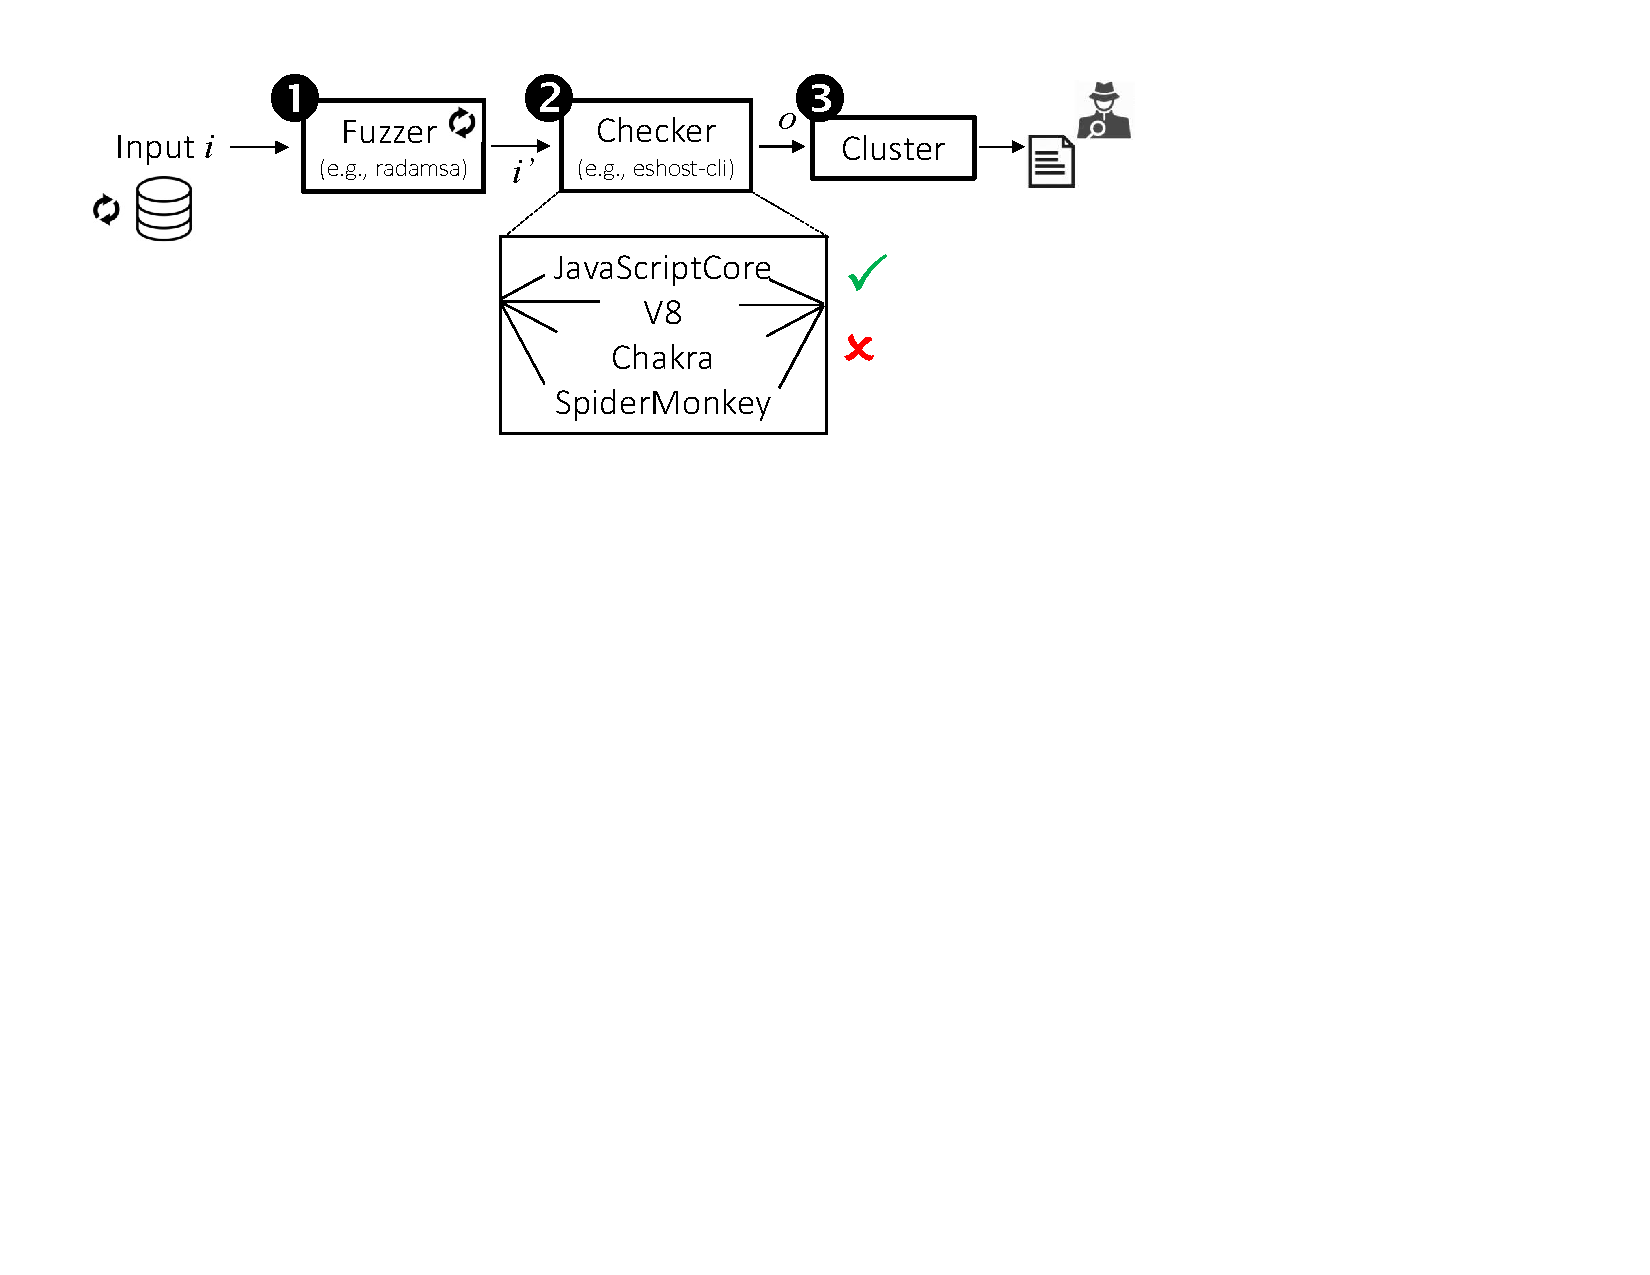
\includegraphics[trim=0 350 150 0,clip,width=1.0\textwidth]{diff-testing-runtimes}
  \vspace{-5ex}
  \caption{\label{fig:workflow}Differential Testing infrastructure overview.}
  \vspace{-2ex}
\end{figure}